%%%%%%%%%%%%%%%%%%%%%%%%%%%%%%%%%%%%%%%%%
% Journal Article
% LaTeX Template
% Version 1.4 (15/5/16)
%
% This template has been downloaded from:
% http://www.LaTeXTemplates.com
%
% Original author:
% Frits Wenneker (http://www.howtotex.com) with extensive modifications by
% Vel (vel@LaTeXTemplates.com)
%
% License:
% CC BY-NC-SA 3.0 (http://creativecommons.org/licenses/by-nc-sa/3.0/)
%
%%%%%%%%%%%%%%%%%%%%%%%%%%%%%%%%%%%%%%%%%

%----------------------------------------------------------------------------------------
%	PACKAGES AND OTHER DOCUMENT CONFIGURATIONS
%----------------------------------------------------------------------------------------

\documentclass[twoside,twocolumn]{article}

\usepackage{blindtext} % Package to generate dummy text throughout this template 

\usepackage[sc]{mathpazo} % Use the Palatino font
\usepackage[T1]{fontenc} % Use 8-bit encoding that has 256 glyphs
\linespread{1.05} % Line spacing - Palatino needs more space between lines
\usepackage{microtype} % Slightly tweak font spacing for aesthetics

\usepackage[english]{babel} % Language hyphenation and typographical rules

\usepackage[hmarginratio=1:1,top=32mm,columnsep=20pt]{geometry} % Document margins
\usepackage[hang, small,labelfont=bf,up,textfont=it,up]{caption} % Custom captions under/above floats in tables or figures
\usepackage{booktabs} % Horizontal rules in tables

\usepackage{lettrine} % The lettrine is the first enlarged letter at the beginning of the text

\usepackage{enumitem} % Customized lists
\setlist[itemize]{noitemsep} % Make itemize lists more compact

\usepackage{abstract} % Allows abstract customization
\renewcommand{\abstractnamefont}{\normalfont\bfseries} % Set the "Abstract" text to bold
\renewcommand{\abstracttextfont}{\normalfont\small\itshape} % Set the abstract itself to small italic text

\usepackage{titlesec} % Allows customization of titles
\renewcommand\thesection{\Roman{section}} % Roman numerals for the sections
\renewcommand\thesubsection{\roman{subsection}} % roman numerals for subsections
\titleformat{\section}[block]{\large\scshape\centering}{\thesection.}{1em}{} % Change the look of the section titles
\titleformat{\subsection}[block]{\large}{\thesubsection.}{1em}{} % Change the look of the section titles

\usepackage{fancyhdr} % Headers and footers
\pagestyle{fancy} % All pages have headers and footers
\fancyhead{} % Blank out the default header
\fancyfoot{} % Blank out the default footer
\fancyhead[C]{Harvey Hughes $\bullet$ October 2017 $\bullet$ Emmanuel College} % Custom header text
\fancyfoot[RO,LE]{\thepage} % Custom footer text

\usepackage{titling} % Customizing the title section

\usepackage{hyperref} % For hyperlinks in the PDF

\usepackage{graphicx}
\graphicspath{ {images/} }

\newenvironment{reusefigure}[2][htbp]
  {\addtocounter{figure}{-1}%
   \renewcommand{\theHfigure}{dupe-fig}% If you're using hyperref
   \renewcommand{\thefigure}{\ref{#2}}% Figure counter is \ref
   \renewcommand{\addcontentsline}[3]{}% Avoid placing figure in LoF
   \begin{figure}[#1]}
  {\end{figure}}
\usepackage{wrapfig}
\usepackage{amsmath}
%----------------------------------------------------------------------------------------
%	TITLE SECTION
%----------------------------------------------------------------------------------------

\setlength{\droptitle}{-4\baselineskip} % Move the title up

\pretitle{\begin{center}\Huge\bfseries} % Article title formatting
\posttitle{\end{center}} % Article title closing formatting
\title{3C5 - Gyroscopic Phenomena} % Article title
\author{%
\\
\textsc{Harvey Hughes} \\
\normalsize Emmanuel College \\ % Your institution
\normalsize Experiment Partner: Cameron Millar \\
\normalsize \href{mailto:hh458@cam.ac.uk}{hh458@cam.ac.uk} % Your email address
}
\date{\today} % Leave empty to omit a date
\renewcommand{\maketitlehookd}{%
\begin{abstract}
\noindent
Coriolis accelerations are hard to imagine as their occurrence day to day is very low. However the forces caused by these accelerations play a key role in applications involving gyroscopes. These applications can be anything from toy gyroscopes to specifying the whole motion of a body through space. By using a gyroscope setup in two ways these applications were investigated, and the results were compared to theoretical calculations. There were slight differences between these due to errors in measurement and physical quantities of the equipment.
\newline
\end{abstract}
}

%----------------------------------------------------------------------------------------

\begin{document}

% Print the title
\maketitle

%----------------------------------------------------------------------------------------
%	ARTICLE CONTENTS
%----------------------------------------------------------------------------------------

\section{Introduction}

\lettrine[nindent=0em,lines=3]{T}he objective of this lab was to observe gyroscopic motion and to relate this back to theory taught in the lecture series. The uses of gyroscopes in the real world were also explored. 
\newline

%------------------------------------------------
\section{Apparatus and Experimental Method}
The experiments consisted of using a 10.8kg gyroscope mounted onto a stand with rotational freedom. The details of this arrangement as well as the experimental method can be located in the '3C5 Gyroscopic Phenomena' handout. 

%------------------------------------------------
\section{Results and Discussion}
\subsection{Preliminary Calculations}
To estimate the moment of inertia 'C' about the axis of rotation, the mass was all assumed to reside 70mm from the rotation axis. The equation $J = \int r^{2}dm = 4.2x0.07^{2} = 0.0207kgm^2$ was used to calculate the inertia, this results in a very close approximation to the value listed in the handout of 0.021$kgm^2$.
To calculate the moment of inertia about the two other principle axis' the perpendicular axis theorem was used which states they should be half the value of C. This is due the second and third axis' inertia being the same, and needing to sum to give C.
\newline
The radius of gyration about pin 1 is calculated using $k=\sqrt{\frac{I_G}{m}}=\sqrt{\frac{0.084}{10.8}}=0.088m$
\newline
In order to calculate the moment of inertia about pin 2 the following equation was used, $I=I_G +Mr^2 = 0.084+0.21^2*10.8 = 0.56kgm^2$


%---------------------------------------
\subsection{Steady Precession}
\begin{figure}[h]
  \centering
    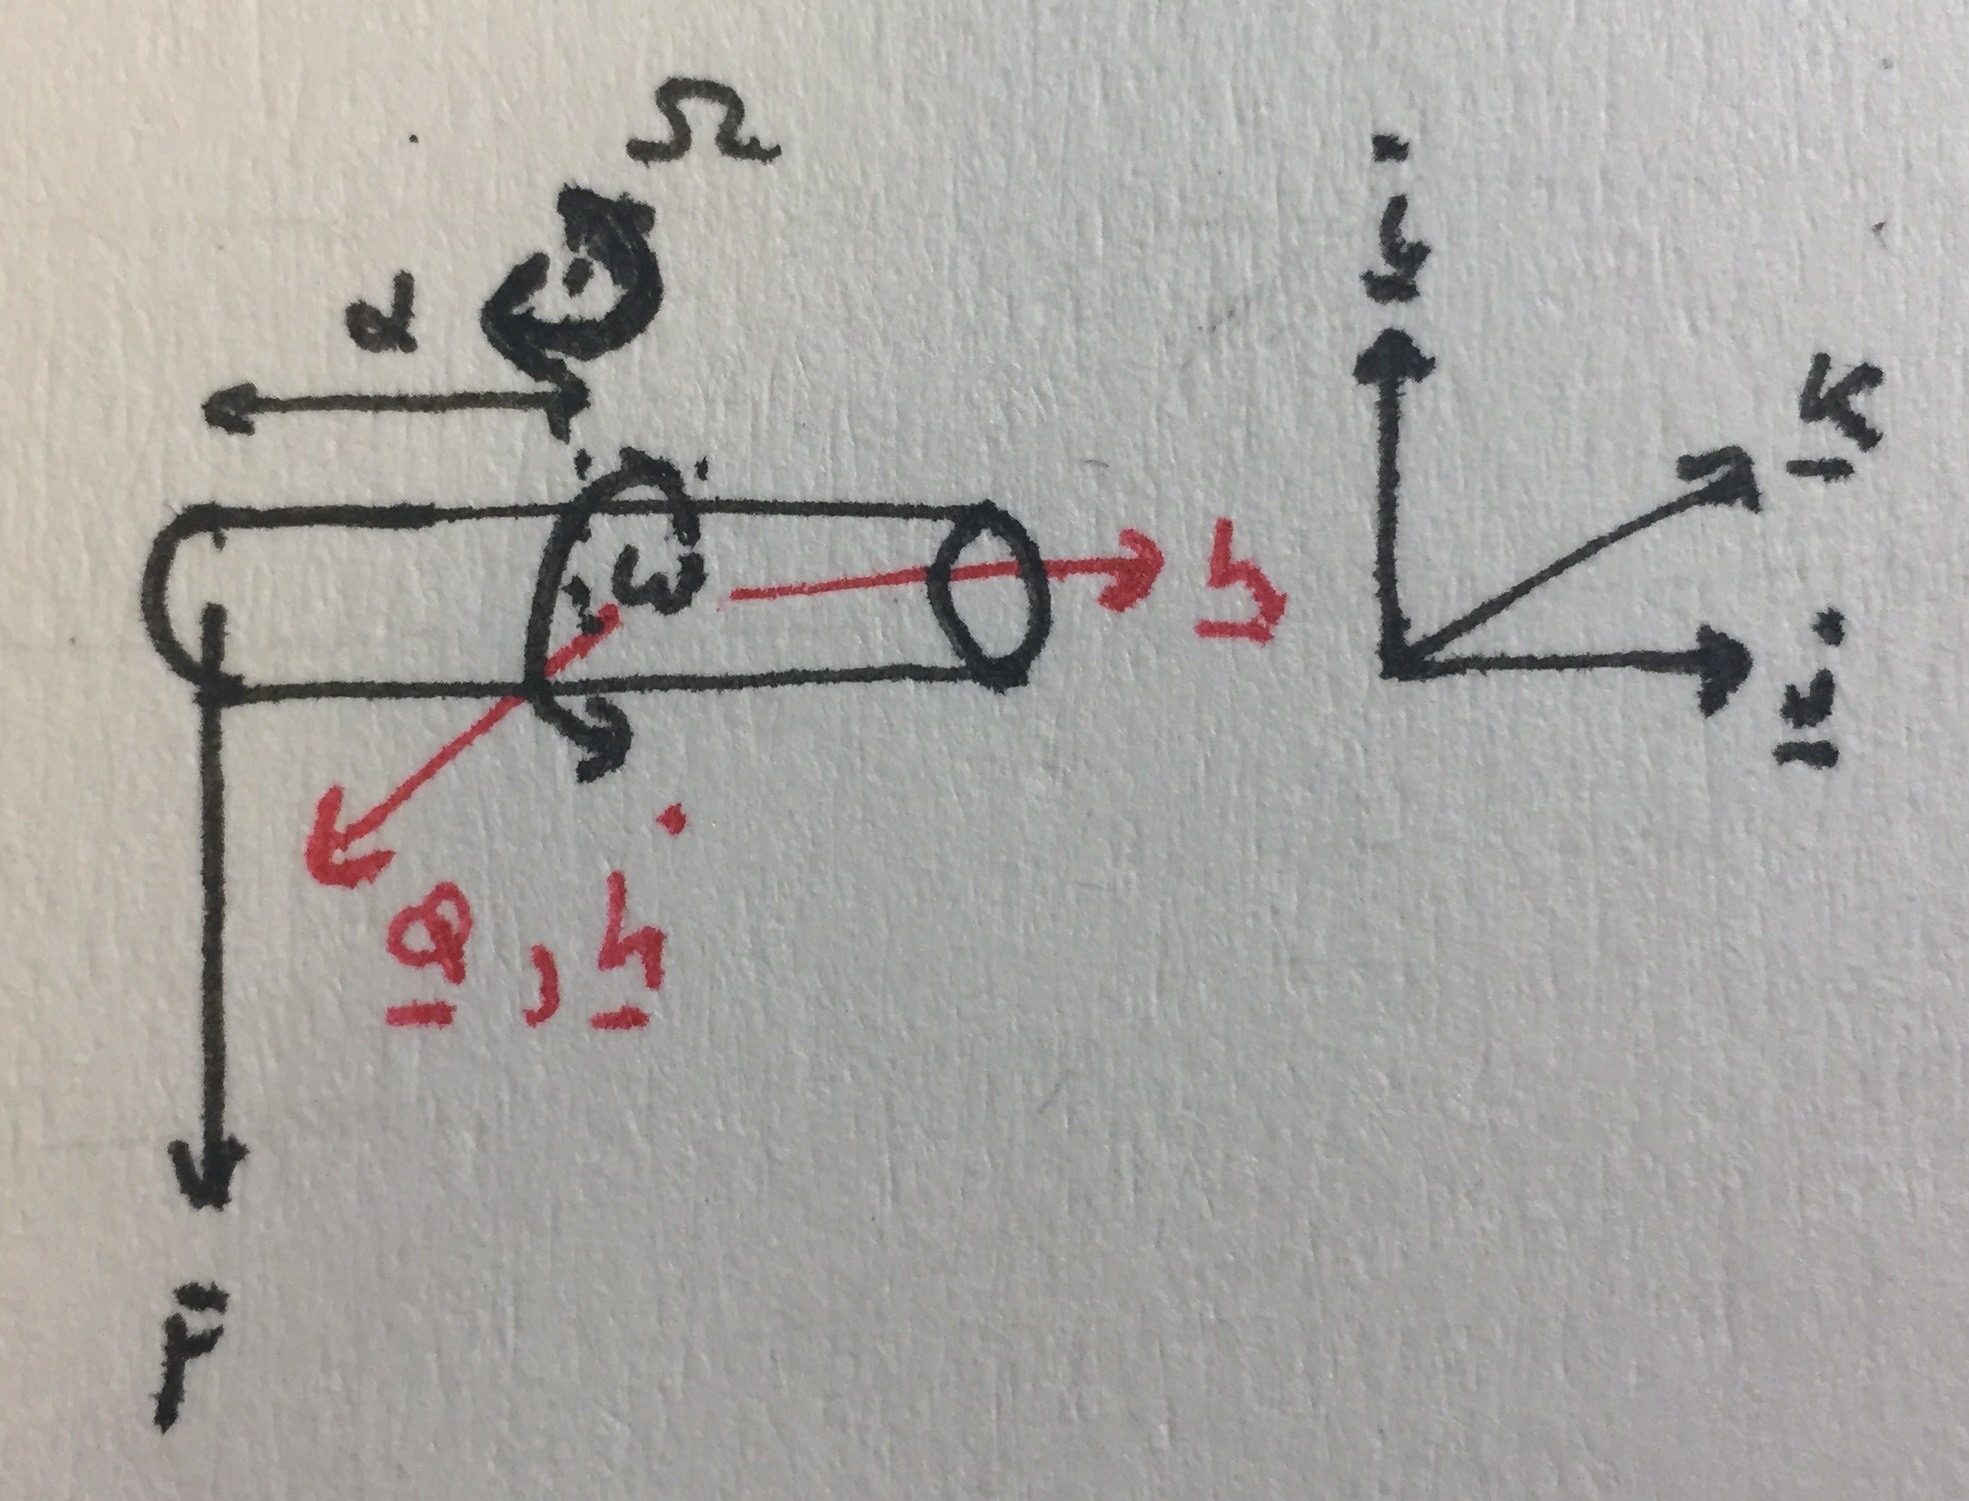
\includegraphics[width=\linewidth]{SPVector}
  \caption{Vector diagram of the steady procession set up}
  \label{fig:spvector}
\end{figure}

In order to work out the direction of precession during this experiment a vector diagram (see figure \ref{fig:spvector}) and equation \ref{eq:1} were used. This gives you a clockwise rotation viewed from above.

\begin{equation}
\label{eq:1}
\begin{split}
&\underline{Q} = \underline{\dot{h}} \\
&\underline{Q} = -Fd\underline{k}\\
&\underline{\dot{h}}=-\Omega\underline{i}xC\omega\underline{j}=-C\omega\Omega\underline{k}\\
&\Omega=-\frac{Fd}{C\omega}\underline{i}\\
\end{split}
\end{equation} 
The 1kg mass is being held up by the reaction acting through the support. The force exerted by the mass is equivalent to its weight and a moment acting around the support as in figure \ref{fig:fbd1}. This weight is opposed by the reaction through the support, with the moment causing gyroscopic precession.

\begin{figure}[h]
  \centering
    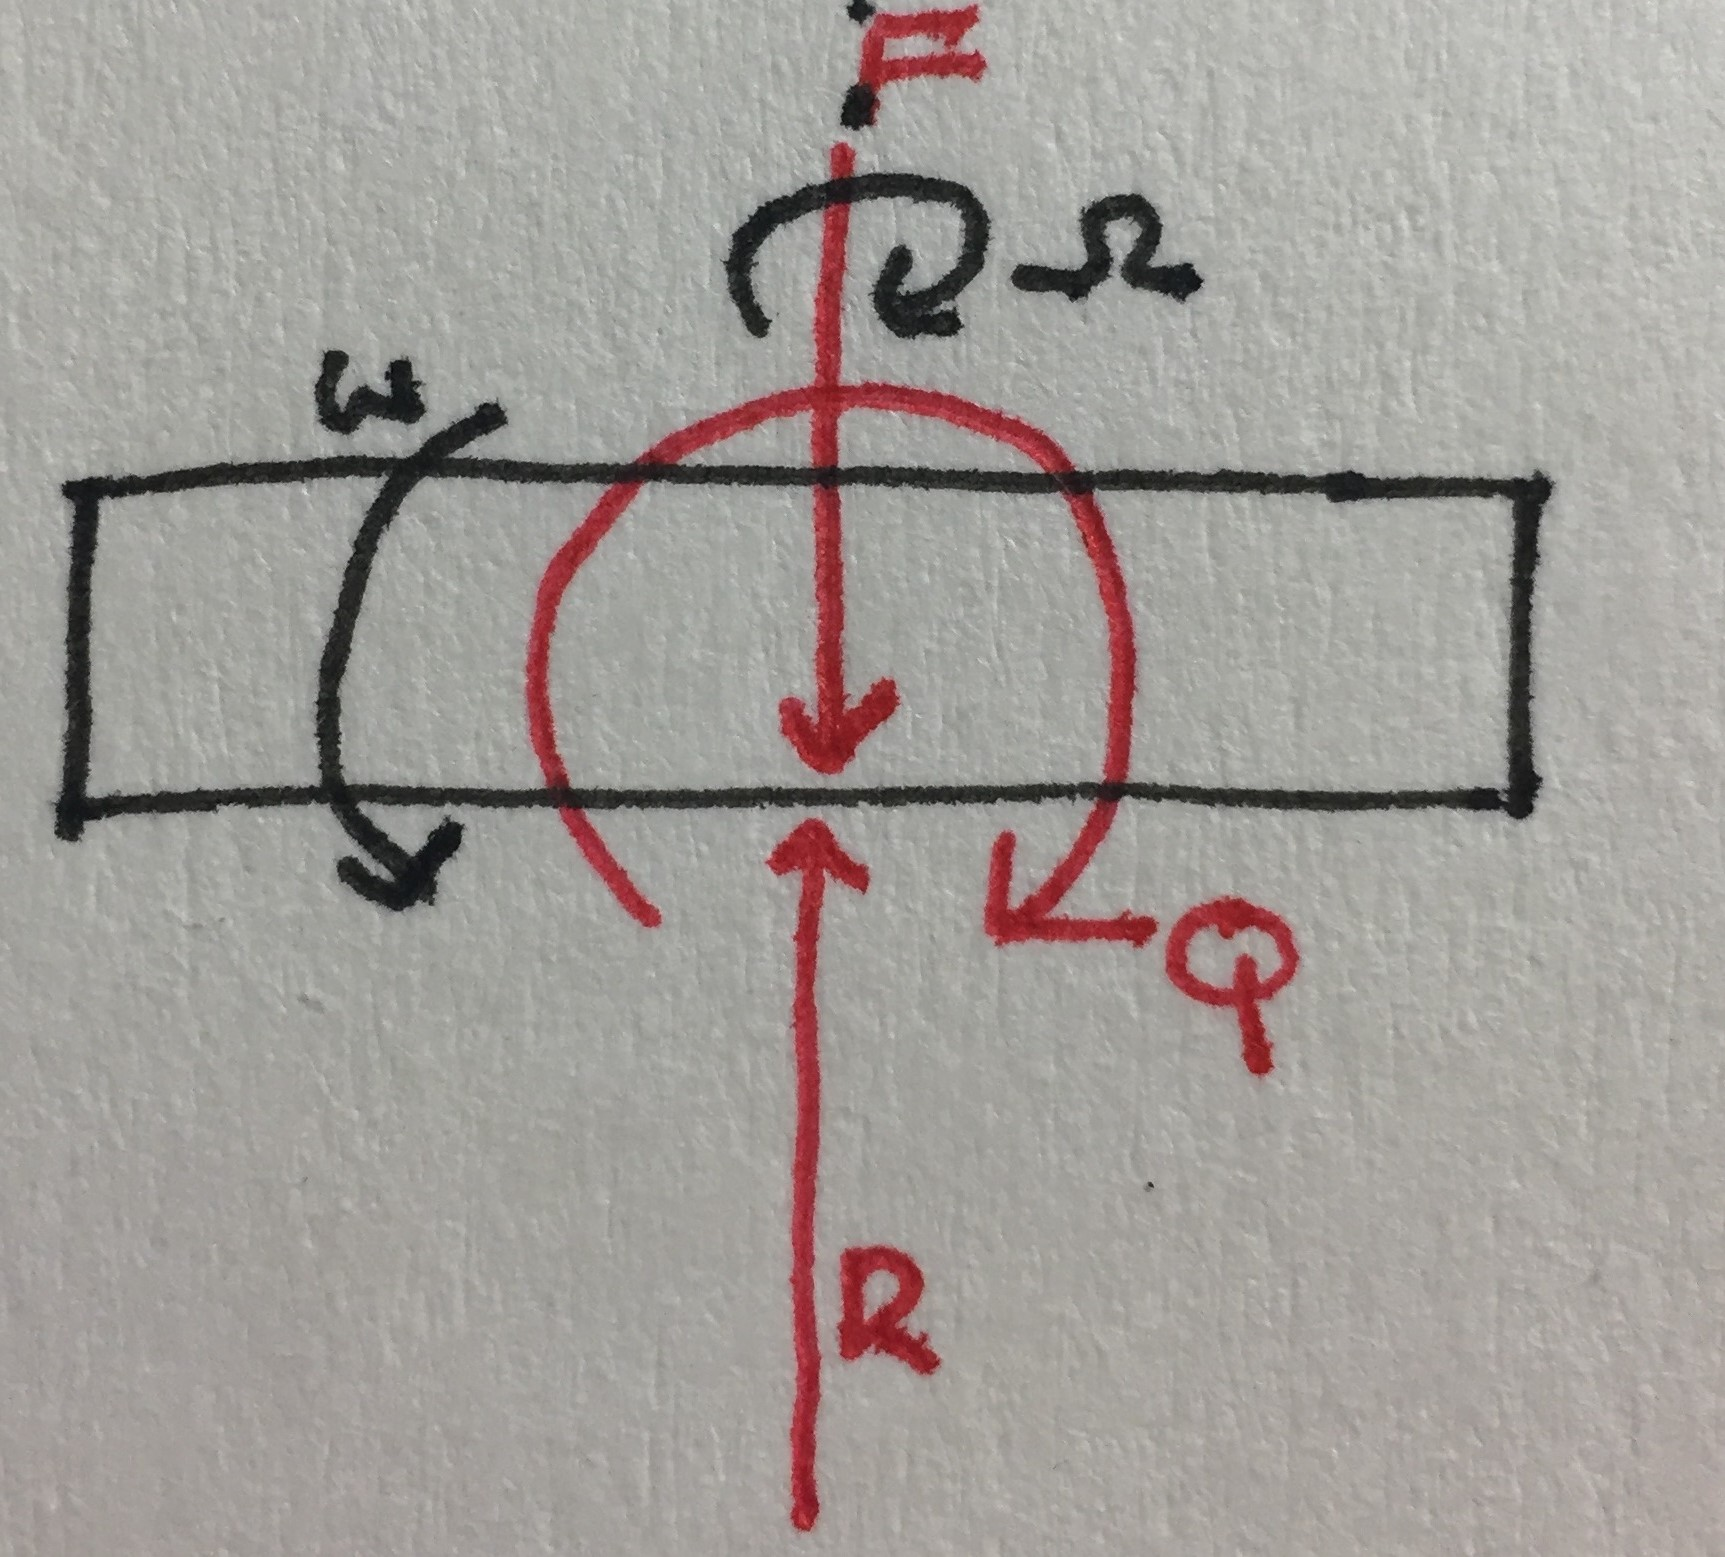
\includegraphics[width=\linewidth]{force}
  \caption{Free body diagram of the gyroscope}
  \label{fig:fbd1}
\end{figure}


Using equation \ref{eq:a4} with the values listed in the lab handout and 5110rpm, a precession rate of $\dot{\phi} = 0.205\frac{rad}{s}$ or 34.27 seconds for one revolution. The disagreement between this and the experimental data in table \ref{table:1} is likely due to imperfect inclination readings. The moment of inertia of the whole system would also be different to the value listed in the handout, further adding error.
 
\begin{equation}
\label{eq:a4}
Q=C\omega\dot{\phi}sin\theta
\end{equation} 
\newline
From equation \ref{eq:a4} it can be seen that for a constant couple, changing the inclination angle would decrease precession time. However, our couple is caused by a mass hung by an arm and therefore is related to $mrsin\theta$, this cancels with the $sin\theta$ in equation \ref{eq:a4}. Therefore,  precession time is independent from inclination angle.  Table \ref{table:1} shows the experimental data agreeing with this within experimental data.

\begin{table}[h]
\caption{Shows the rate of steady precession varying with gyroscope inclination, this precession is caused by a 1kg hung mass.}
\centering
\begin{tabular}{ c | c | c }
Inclination & Precession & Rotor Speed \\
/degrees & Time/s & /rpm  \\
\midrule
90 & 34 & 5110  \\
30 & 27 & 4950 \\
45 & 33 & 5000 \\
120 & 32 & 5160 \\
\end{tabular}
\label{table:1}
\end{table}

Using a mass of 2kg should half the procession time as the couple has twice the magnitude to before. In our experiment we recorded a time of 16 seconds.

%---------------------------------------
\subsection{Nutation}
Nutation frequency can be calculated using equation \ref{eq:nf}, where the first equation is inaccurate due to ignoring the whole gyroscope inertia. For all inclination this gives 20.8Hz nutation frequency. The second equation corrects for the systems inertia, calculated nutation frequencies are   listed in table \ref{table:2}. These calculated frequencies match the measured values closely at low angles.
\begin{equation}
\label{eq:nf}
\begin{split}
&p=\frac{C\omega}{A} \\
&p=\frac{C\omega}{A}/\sqrt{1+\frac{J_1}{A}Cot^2\theta+\frac{I_1}{A}cosec^2\theta}\\
\end{split}
\end{equation} 

\begin{table}[h]
\caption{Shows the nutation frequency varying with gyroscope inclination}
\centering
\begin{tabular}{ c | c | c }
Inclination & Nutation & Theoretical \\
/degrees & Frequency/Hz &Frequency/Hz \\
\midrule
90 & 21.4 & 19.1  \\
60 & 20.1 & 18.1 \\
45 & 16.8 &16.6 \\
30 & 13.2 &13.8 \\
\end{tabular}
\label{table:2}
\end{table}


%----------------------------------------
\subsection{The Rate Gyro}
By attaching springs to the assembly (see figure \ref{fig:rate}) a couple which varies with gyroscope inclination was created. The couple acting on the rotor can be calculated using \ref{eq:a4} with a rpm of 5000. These are tabulated in table \ref{table:3}. The springs are approximately 60mm from the pins, therefore a force difference can be calculated between the two springs, Equation \ref{eq:fd} is used here. Due to the pretension of both springs when horizontal and not measuring spring length only the force difference can be calculated. The length difference between the springs is $0.12cos\theta$ using a spring constant of 500N/m results in force differences of 42.4, 30 and 15.6N for each inclination. These values are approximately 2.8 times smaller than table \ref{table:3}. This difference is likely due to a different spring constant and distance present in the apparatus.

\begin{figure}[h]
  \centering
    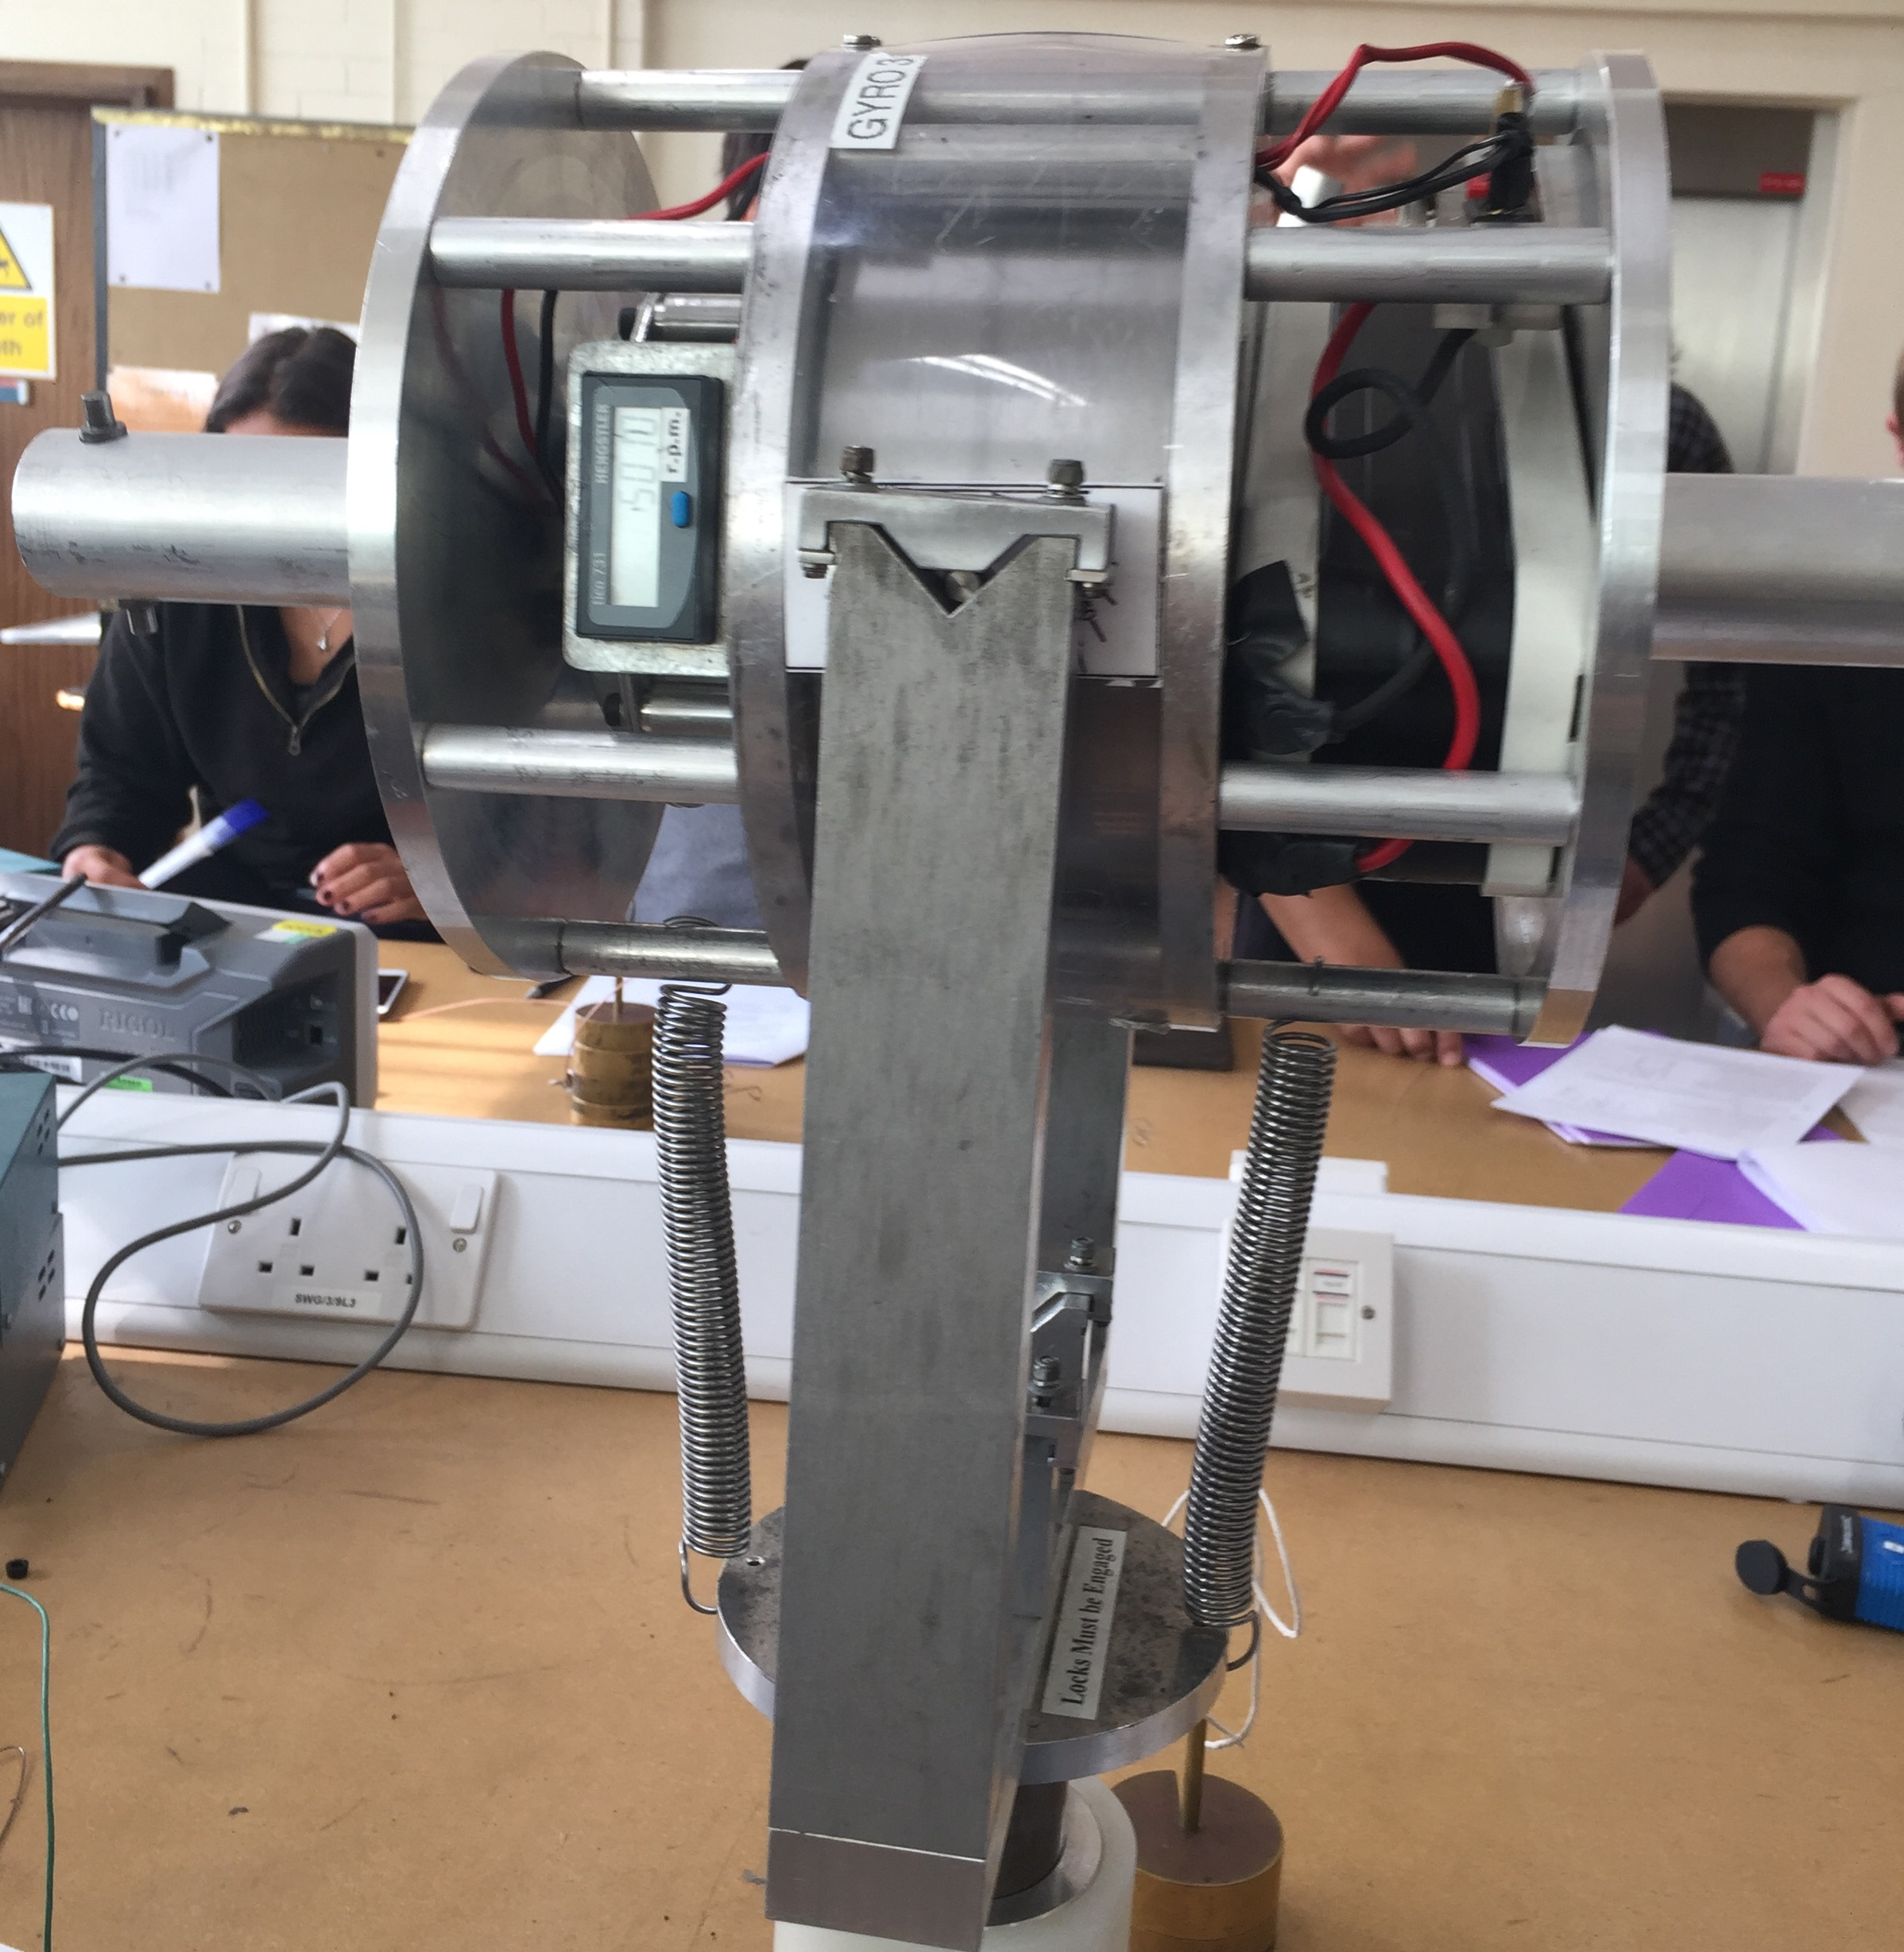
\includegraphics[width=\linewidth]{rg}
  \caption{Experimental set up of the rate gyro}
  \label{fig:rate}
\end{figure}

\begin{equation}
\label{eq:fd}
0.06(F_1-F_2) = Q
\end{equation} 

\begin{table}[h]
\caption{Shows the precession rate created with two springs attached at various inclinations}
\centering
\begin{tabular}{ c | c | c | c }
Inclination & Precession & Couple &$F_1-F_2$ \\
/degrees & Time/s & /Nm &/N \\
\midrule
135 & 6.9 & 7.1 &118 \\
120 & 10.8 & 5.5 &92 \\
75 & 30.7 & 2.2 & 36 \\
\end{tabular}
\label{table:3}
\end{table}

This rate gyro can be used to measure rotation of the boat. The rotation will cause a moment to be generated in the gyro which can be measured to determine how the boat is turning.
\newline
If the gyro is impacted when precessing then nutation will still occur. Nutation is the transient response to an impact and will be present under any condition. Precession is the steady state response caused by the input of a couple. The gyroscope is a linear system, therefore these two separate responses can be added linearly and both occur simultaneously. 

%---------------------------------------
\subsection{Gyroscopic Pendulum}
The forces can once again be moved into a couple and force acting through the support as in figure \ref{fig:fbd1}. With the support reaction opposes the weight and the couple causes gyroscopic precession and with rate calculated using equation \ref{eq:1}. Equations \ref{eq:1} and \ref{eq:couple} with M=10.8kg and l=0.21m are used to obtain a period of precession of 3.17s. This value agrees closely with the recorded data. In order to improve accuracy in measuring time, ten rotations were recorded together.

\begin{equation}
\label{eq:couple}
Q=Mglsin\theta
\end{equation} 

\begin{table}[h]
\caption{Shows how precession time depends on inclination angle from vertical in set up 2}
\centering
\begin{tabular}{ c | c }
Inclination & Precession \\
/degrees & Time/s\\
\midrule
90 & 3.0   \\
45 & 2.8  \\
15 & 2.7  \\
\end{tabular}
\label{table:4}
\end{table}

Nutation can still occur during precession as discussed earlier. The frequency of the oscillations was recorded using a slow motion camera and five wavelengths in order to increase accuracy. Using equation \ref{eq:nf} you can once again get a theoretical prediction of this frequency , see table \ref{table:5}. This prediction agrees with the observed motion very well.

\begin{table}[h]
\caption{Shows how nutation frequency changes with inclination angle for set up 2}
\centering
\begin{tabular}{ c | c | c }
Inclination & Nutation &Calculated \\
/degrees & Frequency/Hz & Frequency/Hz\\
\midrule
90 & 3.13 & 3.08 \\
45 & 2.5 & 3.00\\
\end{tabular}
\label{table:5}
\end{table}

When released from rest cuspidal motion is observed. The energy required to rotate the gyroscope is due to the drop in height of the gyroscope as precession occurs. For total energy to be conserved in equation \ref{eq:energy} potential energy must be converted into kinetic energy for motion to occur.

\begin{equation}
\label{eq:energy}
Total Energy = Kinetic Energy + Potential Energy 
\end{equation} 

The motion is once again caused by the moment exerted on the supports and the change of moment of momentum. The damping throughout the system causes these oscillations to diminish until the gyroscope is in steady state and precessing. This steady state occurs at an inclination less than 90 degrees. This end inclination was too small to measure in the experiment but can be calculated using equation \ref{eq:angle}, resulting in 0.106rad or 6 degrees.

\begin{equation}
\label{eq:angle}
\alpha = \frac{mgr(A+I_1)}{(C\omega)^2}
\end{equation} 

The damping of the system resulted in the observed motion differing to the theory in two regards. The sharp peak at the top of the motion appeared as more of a loop and was a lot smoother. The inclination loss at steady state appeared larger due to the energy losses.
%----------------------------------------
\section{Conclusion}
The theory and experimental observations matched up reasonably well throughout the tests. Differences between them can be accounted to various measurement errors. The inertias of the equipment would all vary from the values listed in the handout due to changes of battery etc. over the years.  Measuring angles was inaccurate to only have large divisions or no divisions to measure from. 


%------------------------------------------------
\end{document}
